\documentclass[aspectratio=169]{beamer}

\usetheme{Boadilla}
\setbeamertemplate{navigation symbols}{}
\setbeamertemplate{footline}{}

\usepackage{booktabs}
\usepackage{graphicx}
\usepackage{tikz}
\usetikzlibrary{arrows.meta,positioning}
\usepackage{array}

\definecolor{navy}{HTML}{102A43}
\definecolor{slate}{HTML}{334455}
\definecolor{blueaccent}{HTML}{0072B2}
\definecolor{vermillion}{HTML}{D55E00}
\definecolor{lightblue}{HTML}{EAF4FA}
\definecolor{lightorange}{HTML}{FFF0E6}
\definecolor{palegray}{HTML}{F5F7FA}

\setbeamercolor{normal text}{fg=slate,bg=white}
\setbeamercolor{frametitle}{fg=navy,bg=white}
\setbeamercolor{title}{fg=navy}
\setbeamercolor{subtitle}{fg=slate}
\setbeamercolor{structure}{fg=blueaccent}
\setbeamerfont{frametitle}{series=\bfseries,size=\Large}
\setbeamerfont{title}{series=\bfseries,size=\huge}
\setbeamerfont{subtitle}{size=\large}
\setbeamerfont{block title}{series=\bfseries}
\setbeamertemplate{itemize item}{\raise0.1ex\hbox{\color{blueaccent}\tiny$\bullet$}}
\setbeamertemplate{itemize subitem}{\raise0.1ex\hbox{\color{vermillion}\tiny$\bullet$}}

\newcommand{\smallnote}[1]{\vspace{0.25em}{\footnotesize\color{slate}#1}}
\newcommand{\metricbox}[3]{%
  \begin{beamercolorbox}[wd=\linewidth,sep=0.75em,rounded=true,shadow=false]{metricbox}
    {\footnotesize\color{slate}#1}\\[-0.15em]
    {\Large\bfseries\color{#3}#2}
  \end{beamercolorbox}
}
\newcommand{\calloutbox}[2]{%
  \begin{beamercolorbox}[wd=\linewidth,sep=0.7em,rounded=true,shadow=false]{callout}
    {\bfseries\color{navy}#1}\\[-0.1em]
    {\footnotesize\color{slate}#2}
  \end{beamercolorbox}
}

\setbeamercolor{metricbox}{bg=palegray,fg=slate}
\setbeamercolor{callout}{bg=lightblue,fg=slate}
\setbeamercolor{alerted text}{fg=vermillion}

\title{metaDEBASS \textemdash{} who do you trust tonight?}
\subtitle{Trust-aware fusion of transient classifiers for Rubin/LSST follow-up}
\author{}
\date{}

\begin{document}

\begin{frame}[plain]
  \vspace{1.1cm}
  {\usebeamerfont{title}\usebeamercolor[fg]{title}\inserttitle\par}
  \vspace{0.35cm}
  {\usebeamerfont{subtitle}\usebeamercolor[fg]{subtitle}\insertsubtitle\par}
  \vfill
  
\begin{tikzpicture}
    \fill[blueaccent] (0,0) rectangle (3.2,0.08);
    \fill[vermillion] (3.35,0) rectangle (4.1,0.08);
    \fill[navy] (4.25,0) rectangle (11.6,0.08);
  \end{tikzpicture}
\end{frame}

\begin{frame}{Problem: early follow-up is a trust problem}
  \begin{columns}[T,totalwidth=\textwidth]
    \begin{column}{0.52\textwidth}
      \begin{itemize}
        \item LSST will deliver $\sim 10\mathrm{M}$ alerts/night scored by many broker classifiers that often disagree.
        \item Follow-up observers need to know \textbf{which classifier to trust on which object}.
        \item The decision has to happen after only \textbf{3--5 detections}.
      \end{itemize}
    \end{column}
    \begin{column}{0.42\textwidth}
      \calloutbox{Primary product}{Per-expert confidence at the current object epoch.}
      \vspace{0.6em}
      \calloutbox{Secondary output}{A trust-weighted follow-up proxy for tonight's science goal.}
      \vspace{0.6em}
      \calloutbox{Truth boundary}{Broker-derived labels stay weak; final science truth stays separate.}
    \end{column}
  \end{columns}
\end{frame}

\begin{frame}{Architecture: confidence first, priority second}
  \centering
  \resizebox{0.96\textwidth}{!}{%
  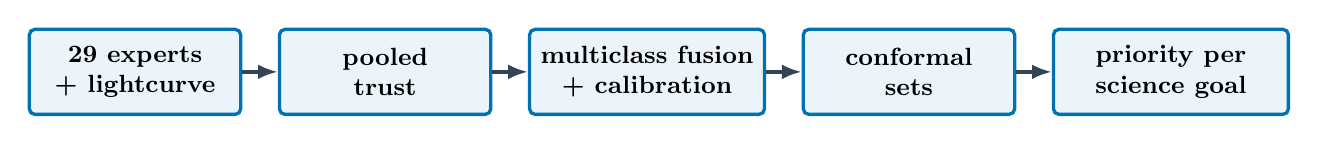
\begin{tikzpicture}[
      node distance=0.45cm,
      flow/.style={
        draw=blueaccent,
        very thick,
        fill=lightblue,
        rounded corners=2pt,
        align=center,
        minimum height=1.08cm,
        text width=2.45cm,
        font=\small\bfseries
      },
      arr/.style={-{Latex[length=2.5mm]},very thick,draw=slate}
    ]
    \node[flow] (experts) {29 experts\\+ lightcurve};
    \node[flow,right=of experts] (trust) {pooled\\trust};
    \node[flow,right=of trust,text width=2.75cm] (fusion) {multiclass fusion\\+ calibration};
    \node[flow,right=of fusion] (sets) {conformal\\sets};
    \node[flow,right=of sets,text width=2.75cm] (priority) {priority per\\science goal};
    \draw[arr] (experts) -- (trust);
    \draw[arr] (trust) -- (fusion);
    \draw[arr] (fusion) -- (sets);
    \draw[arr] (sets) -- (priority);
  \end{tikzpicture}
  }

  \vspace{0.85em}
  \begin{columns}[T,totalwidth=\textwidth]
    \begin{column}{0.46\textwidth}
      \calloutbox{Expert confidence}{Learn $P(\mathrm{expert\ right}\mid \mathrm{object}, \mathrm{epoch})$ before asking for a fused class.}
    \end{column}
    \begin{column}{0.46\textwidth}
      \calloutbox{Goal conditioning}{Rank with $u\cdot p$ after calibration and abstain when conformal sets stay broad.}
    \end{column}
  \end{columns}
\end{frame}

\begin{frame}{Honesty machinery}
  \begin{columns}[T,totalwidth=\textwidth]
    \begin{column}{0.55\textwidth}
      \begin{itemize}
        \item Pre-registered headline and guards.
        \item Locked test split byte-identical across versions.
        \item Component gates decided on calibration with bootstrap CIs.
        \item Label-provenance anti-circularity: weak labels are not science truth.
        \item Independent audits: adversarial re-computation and code audit.
      \end{itemize}
      \smallnote{Headline protocol: object-level, spectroscopic-only, locked test split, n\_det=5, 1000-resample paired object bootstrap.}
    \end{column}
    \begin{column}{0.38\textwidth}
      \begin{beamercolorbox}[wd=\linewidth,sep=0.95em,rounded=true,shadow=false]{metricbox}
        {\footnotesize\color{slate}Label provenance bug fixed}\\[0.15em]
        {\Huge\bfseries\color{vermillion}3,149}\\[-0.15em]
        {\footnotesize\color{slate}BTS-unclassified objects carried fabricated nonIa/spectroscopic labels.}\\[0.4em]
        {\Large\bfseries\color{navy}15}\\[-0.1em]
        {\footnotesize\color{slate}were in the locked test; all were demoted.}
      \end{beamercolorbox}
    \end{column}
  \end{columns}
\end{frame}

\begin{frame}{Headline: pre-registered gain over the previous system}
  \begin{columns}[T,totalwidth=\textwidth]
    \begin{column}{0.68\textwidth}
      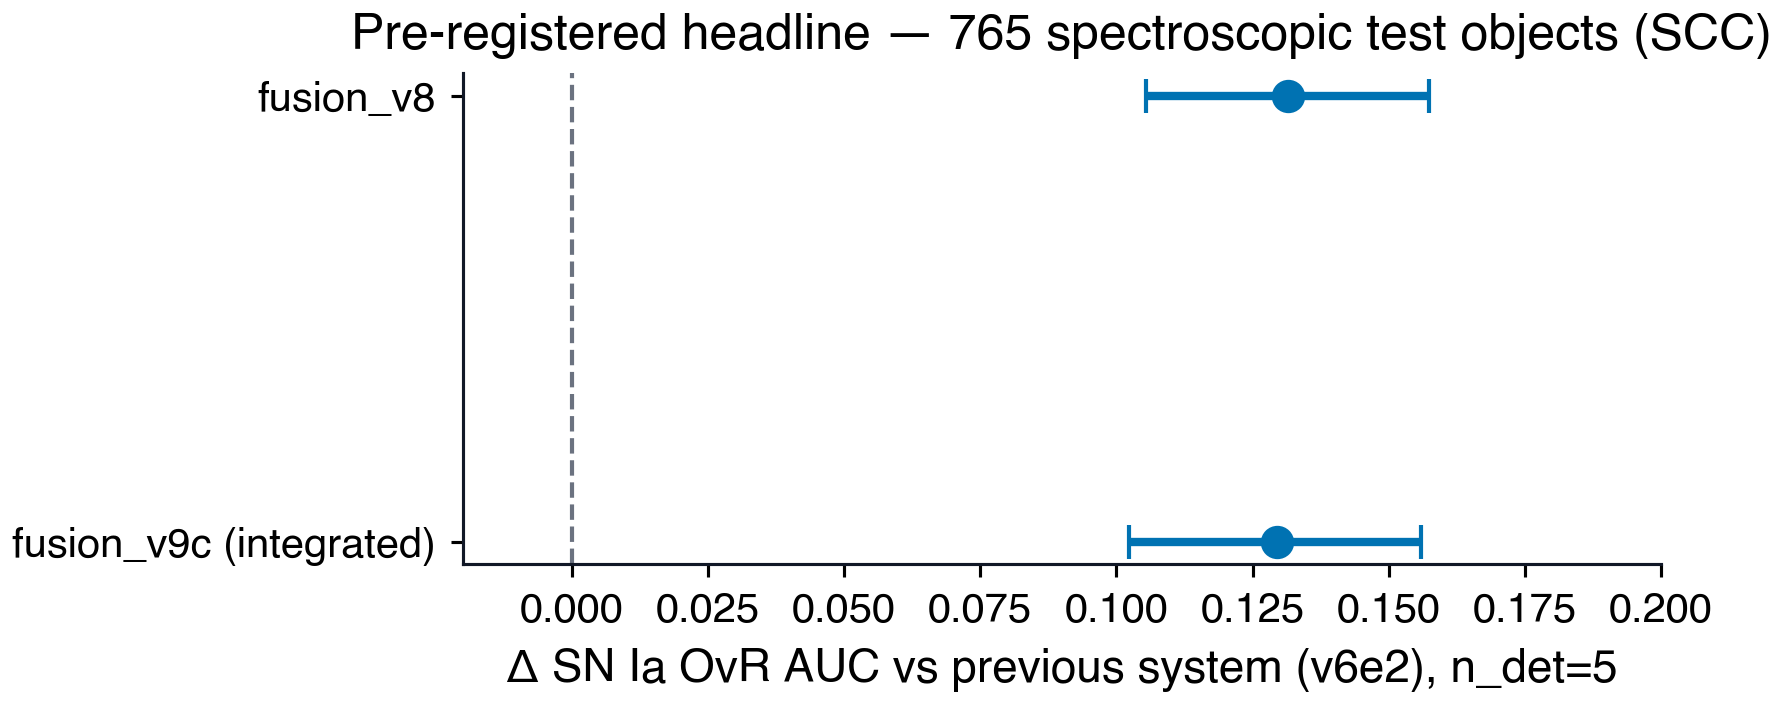
\includegraphics[width=\linewidth]{../figs/fig_headline.png}
      \smallnote{Object-level, spectroscopic-only, locked test, n\_det=5.}
    \end{column}
    \begin{column}{0.28\textwidth}
      \metricbox{Delta SN Ia OvR AUC}{+0.129 [0.102, 0.156]}{blueaccent}
      \vspace{0.55em}
      \metricbox{Spectroscopic test objects}{765}{navy}
      \vspace{0.55em}
      \metricbox{Macro AUC}{0.921}{vermillion}
    \end{column}
  \end{columns}
\end{frame}

\begin{frame}{AUC vs n\_det: early-epoch gains persist}
  \begin{columns}[T,totalwidth=\textwidth]
    \begin{column}{0.72\textwidth}
      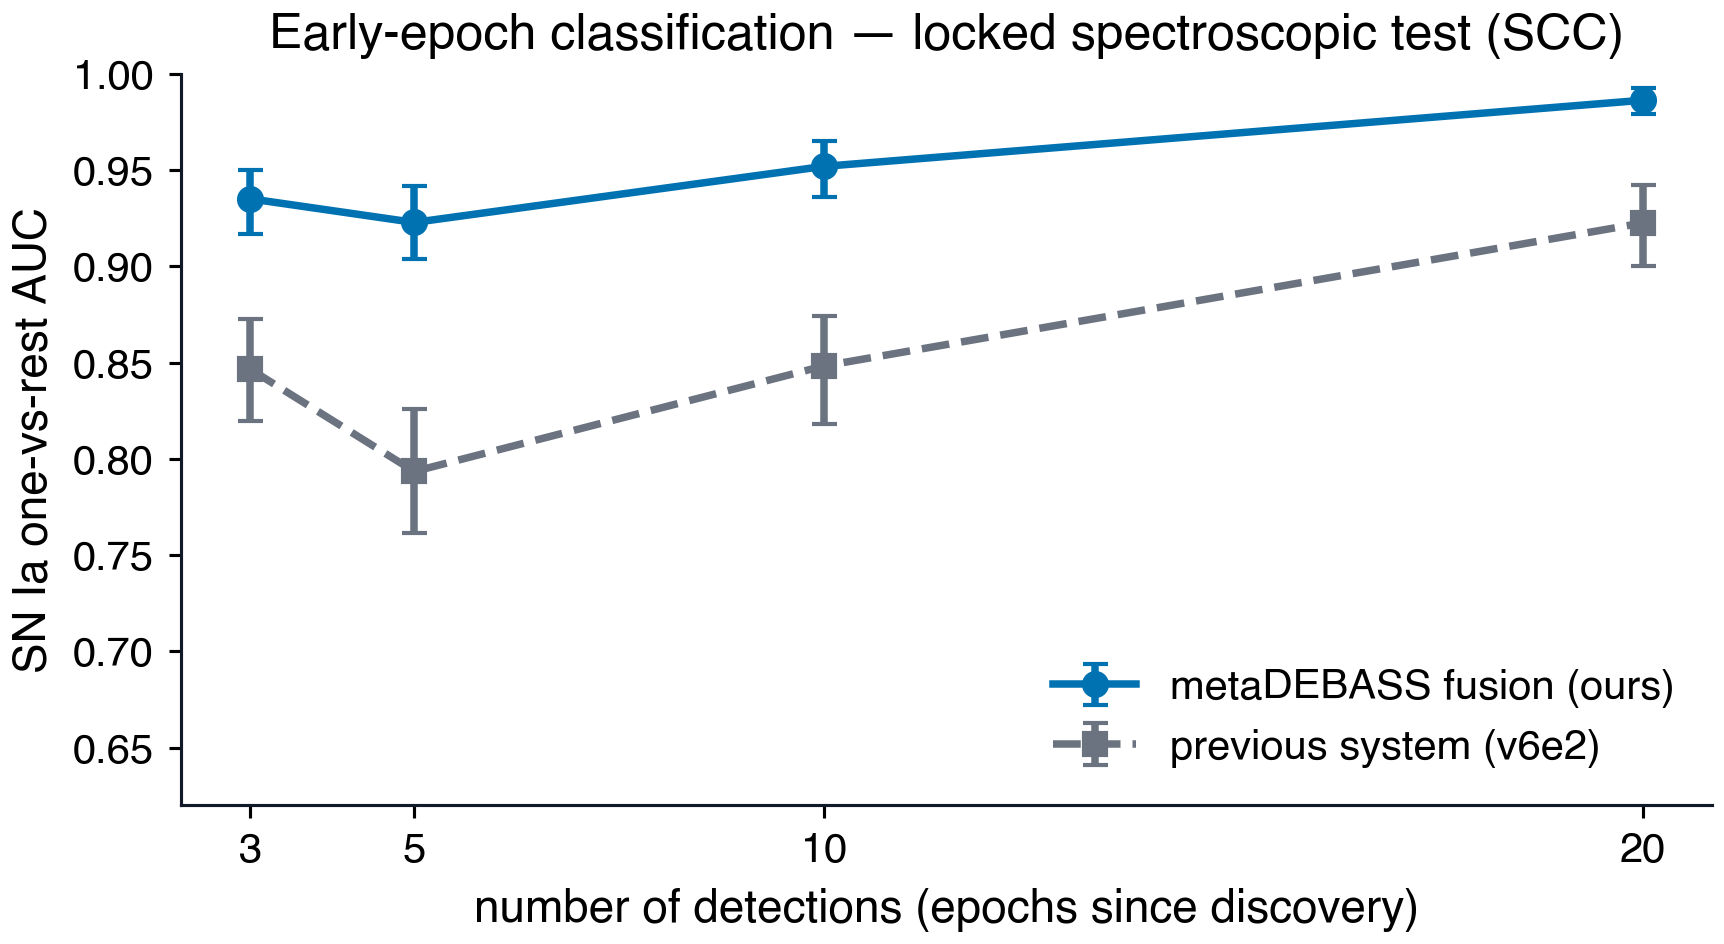
\includegraphics[width=\linewidth]{../figs/fig_auc_vs_ndet.png}
    \end{column}
    \begin{column}{0.24\textwidth}
      \calloutbox{At n\_det=5}{SN Ia OvR AUC is 0.923 vs 0.793 for the previous system.}
      \vspace{0.55em}
      \calloutbox{At n\_det=20}{SN Ia OvR AUC is 0.986 vs 0.923.}
      \vspace{0.55em}
      \calloutbox{Epoch grid}{n\_det values: 3, 5, 10, 20.}
    \end{column}
  \end{columns}
\end{frame}

\begin{frame}{DP1 enrichment: rank for science, expose contaminants}
  \begin{columns}[T,totalwidth=\textwidth]
    \begin{column}{0.70\textwidth}
      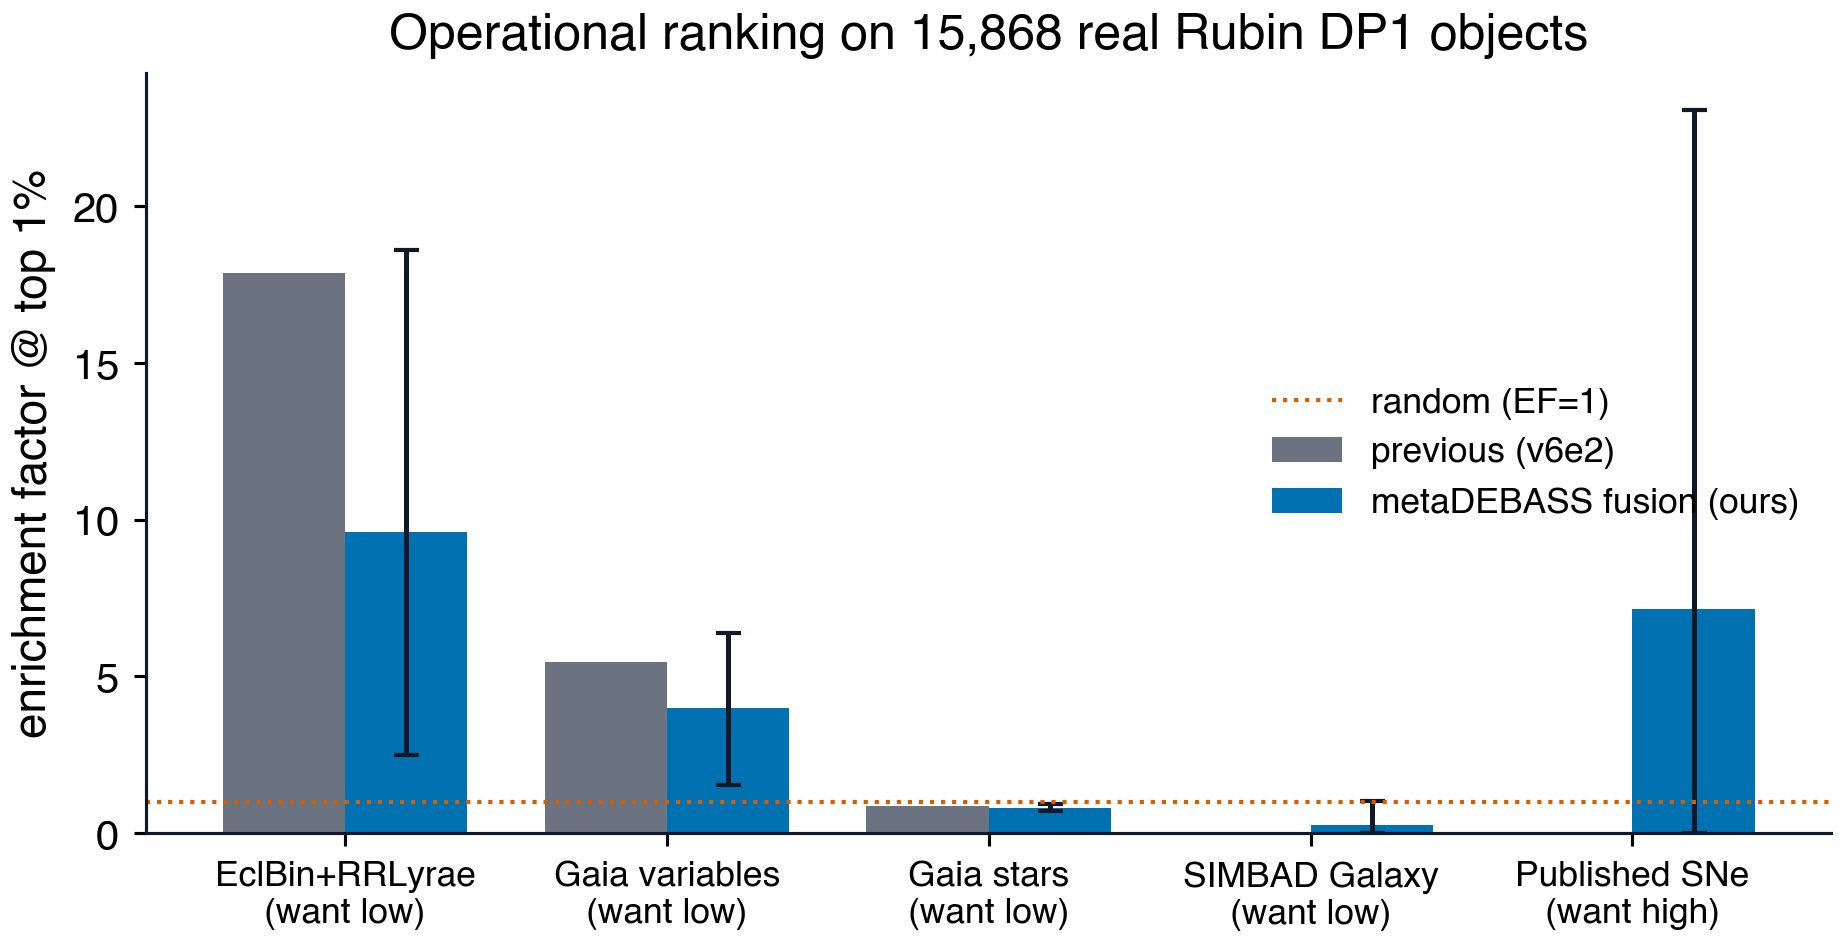
\includegraphics[width=\linewidth]{../figs/fig_dp1_ef.png}
      \smallnote{EF=1 is random; contaminant classes want low, Published SNe wants high. N=15,868 DP1 objects.}
    \end{column}
    \begin{column}{0.26\textwidth}
      \metricbox{EclBin+RRLyrae}{17.9 $\rightarrow$ 9.6}{vermillion}
      \vspace{0.55em}
      \metricbox{Gaia variables}{5.5 $\rightarrow$ 4.0}{vermillion}
      \vspace{0.55em}
      \metricbox{Published SNe}{0.0 $\rightarrow$ 7.1}{blueaccent}
    \end{column}
  \end{columns}
\end{frame}

\begin{frame}{Trust heads: per-expert confidence is learnable}
  \centering
  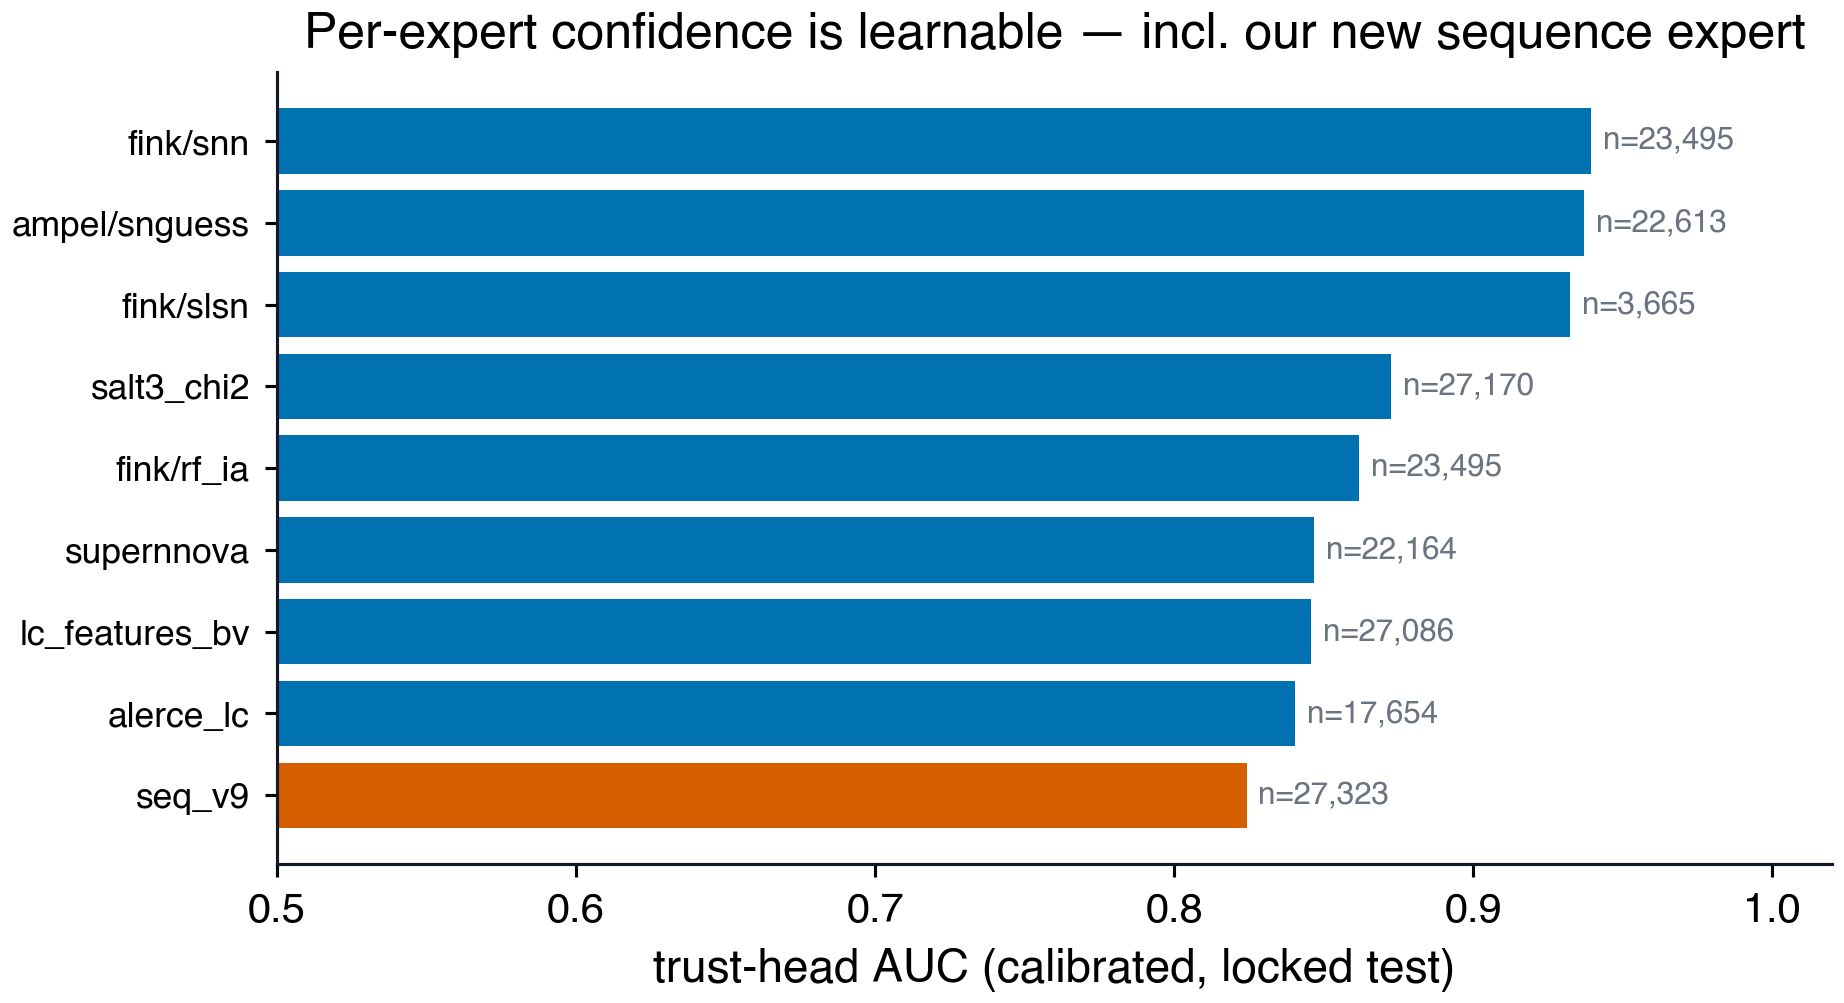
\includegraphics[width=0.86\textwidth,height=0.58\textheight,keepaspectratio]{../figs/fig_trust_heads.png}
  \vspace{0.25em}

  \begin{columns}[T,totalwidth=0.86\textwidth]
    \begin{column}{0.42\textwidth}
      \calloutbox{seq\_v9 highlighted}{Trust-head AUC 0.824 on 27,323 locked-test rows.}
    \end{column}
    \begin{column}{0.42\textwidth}
      \calloutbox{Coverage}{13 trust-headed experts out of 29 registered experts.}
    \end{column}
  \end{columns}
\end{frame}

\begin{frame}{The v9 sequence expert}
  \begin{columns}[T,totalwidth=\textwidth]
    \begin{column}{0.50\textwidth}
      \resizebox{0.98\linewidth}{!}{%
      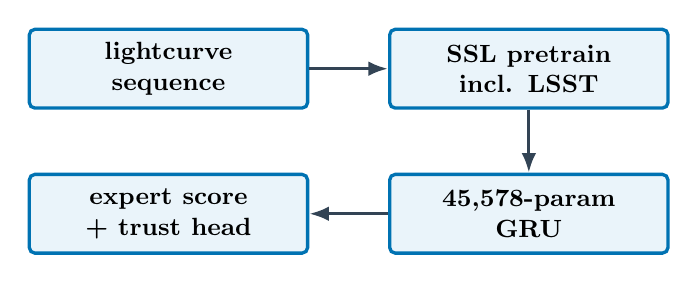
\begin{tikzpicture}[
          block/.style={
            draw=blueaccent,
            very thick,
            fill=lightblue,
            rounded corners=2pt,
            align=center,
            text width=3.3cm,
            minimum height=1.0cm,
            font=\small\bfseries
          },
          arr/.style={-{Latex[length=2.5mm]},very thick,draw=slate}
        ]
        \node[block] (lc) {lightcurve\\sequence};
        \node[block,right=1.0cm of lc] (ssl) {SSL pretrain\\incl. LSST};
        \node[block,below=0.8cm of ssl] (gru) {45,578-param\\GRU};
        \node[block,left=1.0cm of gru] (trust) {expert score\\+ trust head};
        \draw[arr] (lc) -- (ssl);
        \draw[arr] (ssl) -- (gru);
        \draw[arr] (gru) -- (trust);
      \end{tikzpicture}
      }
    \end{column}
    \begin{column}{0.44\textwidth}
      \metricbox{Standalone AUC at n\_det=5}{0.856 / 0.865}{blueaccent}
      \vspace{0.55em}
      \metricbox{Trust-head coverage}{27,323 test rows}{navy}
      \vspace{0.55em}
      \calloutbox{Role in fusion}{Useful as a calibrated trust signal; fusion gate still reports its standalone component result.}
    \end{column}
  \end{columns}
\end{frame}

\begin{frame}{Gate ledger: we report what failed}
  \scriptsize
  \setlength{\tabcolsep}{3pt}
  \renewcommand{\arraystretch}{1.12}
  \begin{tabular}{>{\raggedright\arraybackslash}p{0.29\textwidth}
                  >{\raggedright\arraybackslash}p{0.15\textwidth}
                  >{\raggedright\arraybackslash}p{0.30\textwidth}
                  >{\raggedright\arraybackslash}p{0.17\textwidth}}
    \toprule
    Component & Decision & Delta macro AUC [CI95] & Readout \\
    \midrule
    seq\_features & skipped & not scored & not promoted \\
    ext\_features & kept & +0.0087 [0.0021, 0.0160] & clear cal gain \\
    seq\_v9\_expert & dropped & -0.0009 [-0.0049, 0.0031] & no cal lift \\
    traj\_features & dropped & +0.0005 [-0.0036, 0.0049] & CI crosses zero \\
    pooled\_trust\_q & dropped & -0.0569 [-0.0734, -0.0391] & harmful \\
    expert\_dropout\_aug & dropped & -0.0025 [-0.0057, 0.0011] & no cal lift \\
    dirichlet\_calibration & kept & no delta & calibration guardrail \\
    \bottomrule
  \end{tabular}
\end{frame}

\begin{frame}{Deliverables and next steps}
  \small
  \begin{columns}[T,totalwidth=\textwidth]
    \begin{column}{0.48\textwidth}
      \calloutbox{Built this week}{Gold snapshots: 211,392 rows across 12,772 objects.}
      \vspace{0.35em}
      \calloutbox{Broker layer}{29 experts registered; 13 have trust heads.}
      \vspace{0.35em}
      \calloutbox{Data scale}{8,774 ZTF objects plus 3,998 LSST objects.}
      \vspace{0.35em}
      \calloutbox{Compute}{v9c rerun: 54 min after v8 at 6.0 SCC hours.}
    \end{column}
    \begin{column}{0.46\textwidth}
      \begin{itemize}
        \item Broaden broker history beyond the ALeRCE-heavy seed set.
        \item Make epoch-safe broker snapshots the default trust-training input.
        \item Convert conformal output into observing policies for different science goals.
        \item Promote sequence components only when calibration gates show positive lift.
      \end{itemize}
    \end{column}
  \end{columns}
\end{frame}

\end{document}
